\section{Testing}
The testing phase of a project is one of the most critical ones, a bad testing
plan can lead to a massive loss of time and money, so it is important to follow
the best practices in order to save time and money.

\subsection{Inspection}
Many researches lead by Aetna Insurance Company, Bell-Northern, Hewlett-Packard,
SmartBear and Nasa, pointed out that code inspection has a massive role in
unveiling defects of the code as well as bugs. Inspection will be done during
the development process, as it can be done before the whole component has been
implemented, but must still be done onto "finished" blocks of code. By
the way code inspection will be done only on back-end components, the front-end
is designed as \emph{thin} so it shouldn't do anything apart from
representation. Moreover, the frameworks that are suggested for the front-end
applications, natively provide analysis and testing tools.

The inspection process will be done as follows:
\begin{itemize}
    \item \textbf{Planning:} choose participants, entry-criteria, schedule
        meeting
    \item \textbf{Overview:} mainly assignment of roles and provide a background
        of the project
    \item \textbf{Preparation}
    \item \textbf{Actual Inspection}
    \item \textbf{Rework:} the developers fix the weaknesses of the code found
        in the inspection
    \item \textbf{Follow-up:} moderator makes sure that all the weaknesses has
        been fixed
    \item \textbf{(Re-inspection):} if considered necessary, the inspection
        process can be repeated, especially if many parts of the code has been
        changed.
\end{itemize}

The actual inspection will be done in several meetings of the inspection team.
As we can find in the researches mentioned above, it is functional to schedule
two daily sessions of two hours each. An idea goal is to inspect approximately
200/250 lines of code per session. Further details on the inspection process can
be found in \cite{smartbear:code-inspection}.

\subsection{Unit and integration testing}
Once a component has been implemented and inspected, it must be unit tested to
make sure it works by itself, then the integration test process can begin. The
various components in the sub-groups will be undergoing integration test
simultaneously. In the following pictures, the component that must be integrated
are shown.

\begin{figure}[ht]
    \centering
    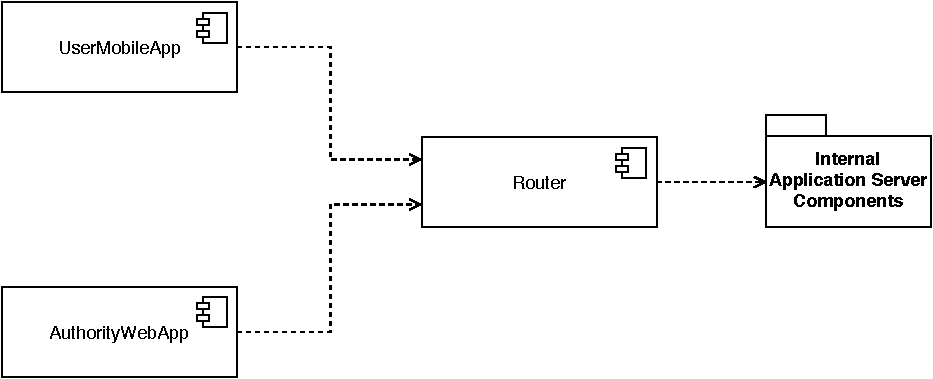
\includegraphics[width=.8\linewidth]{integration_router}
    \caption{Integration testing for the Router}
    \label{fig:integration_router}
\end{figure}

\begin{figure}[ht]
    \centering
    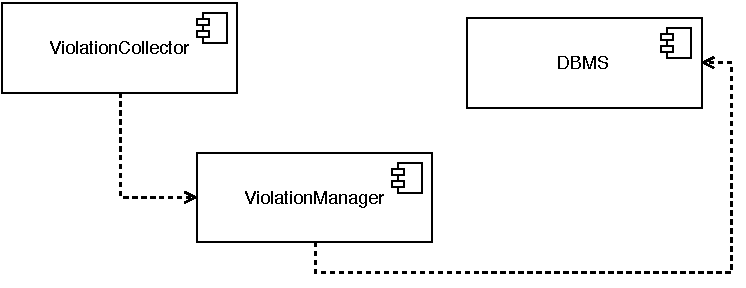
\includegraphics[width=.75\linewidth]{integration_violation}
    \caption{Integration testing for Violation components}
    \label{fig:integration_violation}
\end{figure}

\begin{figure}[ht]
    \centering
    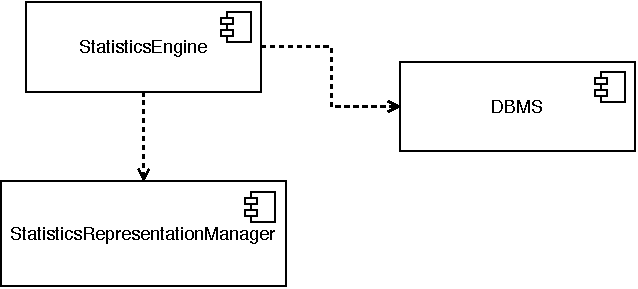
\includegraphics[width=.65\linewidth]{integration_statistics}
    \caption{Integration testing for statistics components}
    \label{fig:integration_statistics}
\end{figure}

\clearpage
\begin{figure}[ht]
    \centering
    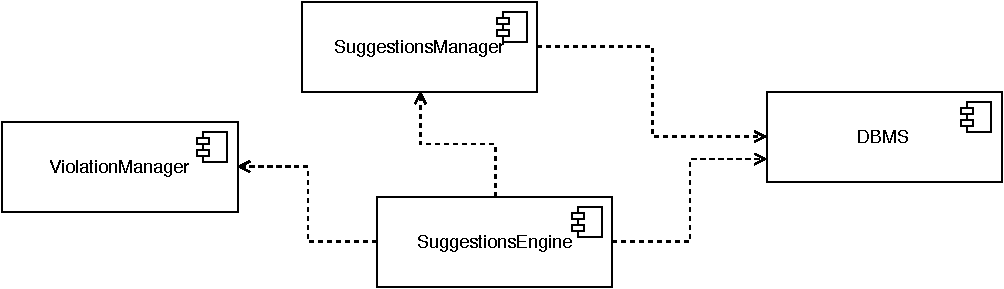
\includegraphics[width=\linewidth]{integration_suggestions}
    \caption{Integration testing for \emph{SmartSuggestions} system}
    \label{fig:integration_suggestions}
\end{figure}

Once all the integration test already shown are done, the entire application
server should be integrated, in other words, a complete integration test with
all the components must be done at this point.